\documentclass[11]{article}

\usepackage[a4paper,left=3cm,right=2cm,top=2.5cm,bottom=2.5cm]{geometry}
\usepackage{lipsum}
\usepackage{amsmath}
\usepackage{multirow}	
\usepackage{graphicx}


\title{Machine Learning HW3}
\author{Payam AZAD - 503111554}
\begin{document}
\pagenumbering{gobble}
 \maketitle
 
 \begin{table}[ht!]
\centering
\label{my-label}
\begin{tabular}{|ll|l|l|l|l|}
\hline
                                             &          & Q1 & Q2 & Q3 & Total \\ \hline
\multicolumn{1}{|l|}{\multirow{2}{*}{Grade}} & Max      & 1  & 2  & 2  &  5     \\ \cline{2-6} 
\multicolumn{1}{|l|}{}                       & Expected & 1  & 2 &   & 3   \\ \hline
\end{tabular}
\end{table}


\section*{Q1}
\subsection*{a}
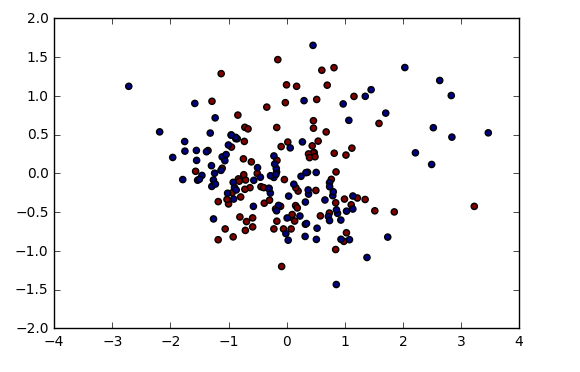
\includegraphics[scale=0.75]{1.png} \\
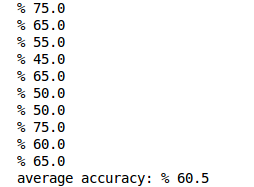
\includegraphics[scale=0.75]{res1.png} \\
\subsection*{b}
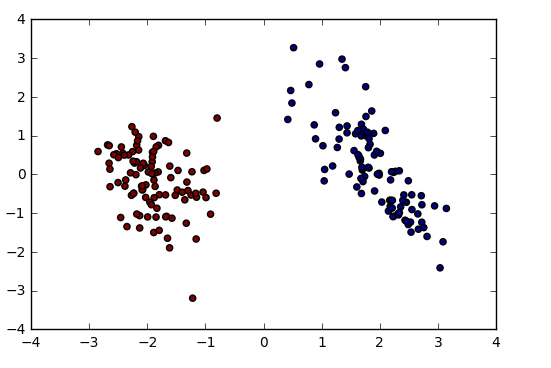
\includegraphics[scale=0.75]{2.png} \\
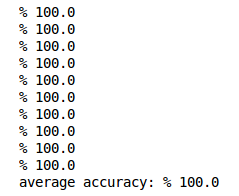
\includegraphics[scale=0.75]{res2.png} \\
When we are mapping features to lower dimension using different classes separately it map features into different principals that are independent of each other. So combining them is pretty meaningless.
 

\section*{Q2}
\subsection*{K=2}
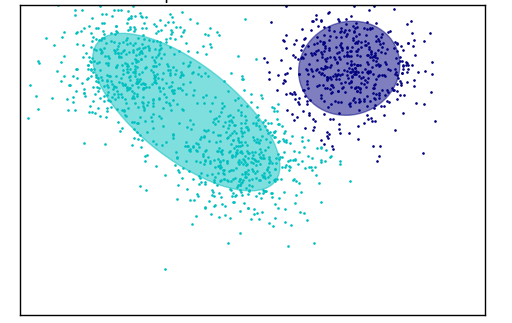
\includegraphics[scale=0.75]{3.png} \\
\subsection*{K=3}
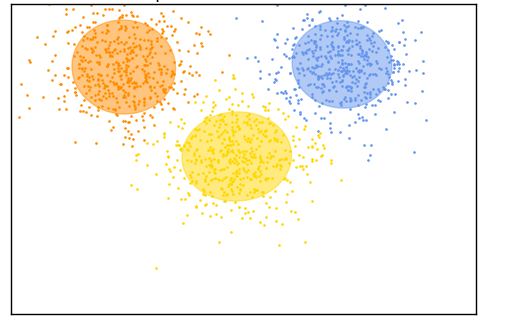
\includegraphics[scale=0.75]{4.png} \\
\subsection*{K=4}
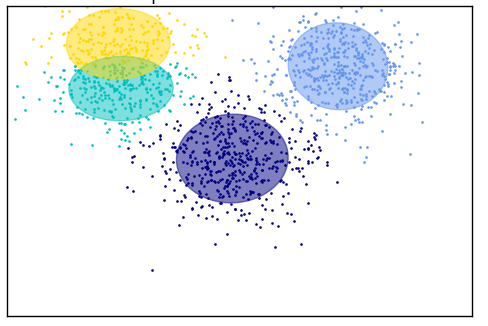
\includegraphics[scale=0.75]{5.png} \\

The best number of clusters was 3.
 



\section*{Q3}




 

\end{document}